\documentclass{article}
\usepackage{graphicx}


\usepackage{hyperref}
\usepackage{xcolor}

\title{REPORT ON PROJECT}
\author{Aryaman Angurana}
\date{June 13, 2023}

\begin{document}

\maketitle

\section*{About the PROJECT}

This project is about making a game in HTML, CSS and Javascript. The game is like minesweeper and cricket.

In this, there is a setup like a board of minesweeper containing points and fielders, like in cricket. The player can choose any box in the board randomly, if it has not been chosen in any previous turn. Then there are two possibilities. If there is a fielder in the cell, the player's turn is over. It is just like the player went to hit and got caught by a fielder. In there is a number, the player earns points(the number that appeared on the board). There are exactly 11 fielders in the grid. The points in the boxes and the placement of fielders are totally random and should not be determined by any factor or trick howsoever. 

\section*{How this game works}

In the game, I have made a first get to go page. In that page, I have given all the instructions for the gameplay- like what the game is, how to play it and all the customization details. In that, at the last, I have added some checkboxes and checklists for the game. The player has to read all the details and then he can begin the game. As the game starts, all the content of the page is gone and a new look appears on the same page. 

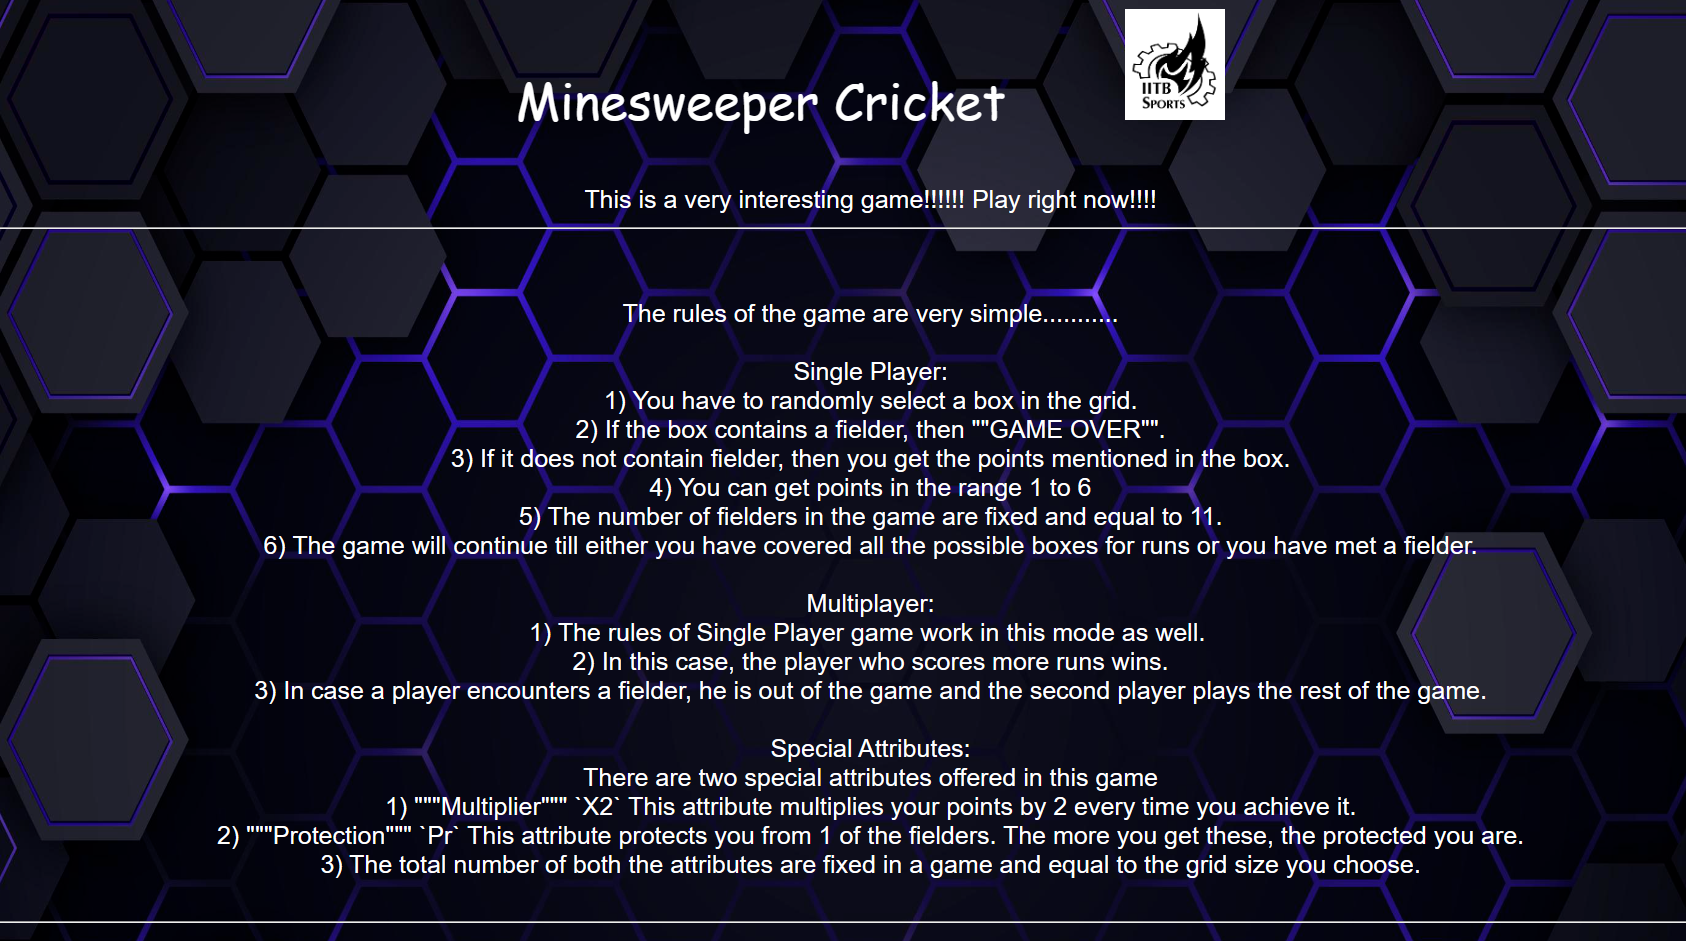
\includegraphics[width=0.8\textwidth]{image1.png}

I took the basic template of the minesweeper code from chatGPT and then worked upon it. I have made a table using javascript and assigned an object to each element of the table, which can have multiple attributes. Then I set the position of the fielders randomly in the table and those cells that did not have any fielders, I gave them a random number as a value. Then I assigned them a function that on clicking the cell, it should call a function by the name revealCell, giving the coordinates of the cell as parameters. Then I checked for the gameover conditions and the points adding conditions in the function; and the game continues in this way.

\section*{Customizations}

In addition to the original project statement, I have added some additional functionalities in the game.

\begin{enumerate}
    \item \textbf{Multiplayer:}
    
    The very first and obvious customization is that I have made the game multiplayer. I made a checklist in the first page, asking the player if he wants to play single player or multiplayer. In multiplayer, I just added another scorecard and alternated the turns of the players. After one of the players got out, I ran the game as a single player game for the other player.

    \item \textbf{Protection:}
    
    In addition to having fielders and points in the cells, I have also added a power, which a player can get if he lands on the cell. This power is PROTECTION. On getting this, the player gets safe if he lands on a fielder. If a player lands on another Protection, he is safe of 2 fielders and so on. For this, I added a new characteristic to the cell, special, in which I can give the name of this special attribute(protect). The number of such cells is limited in the game and is equal to the grid size.
    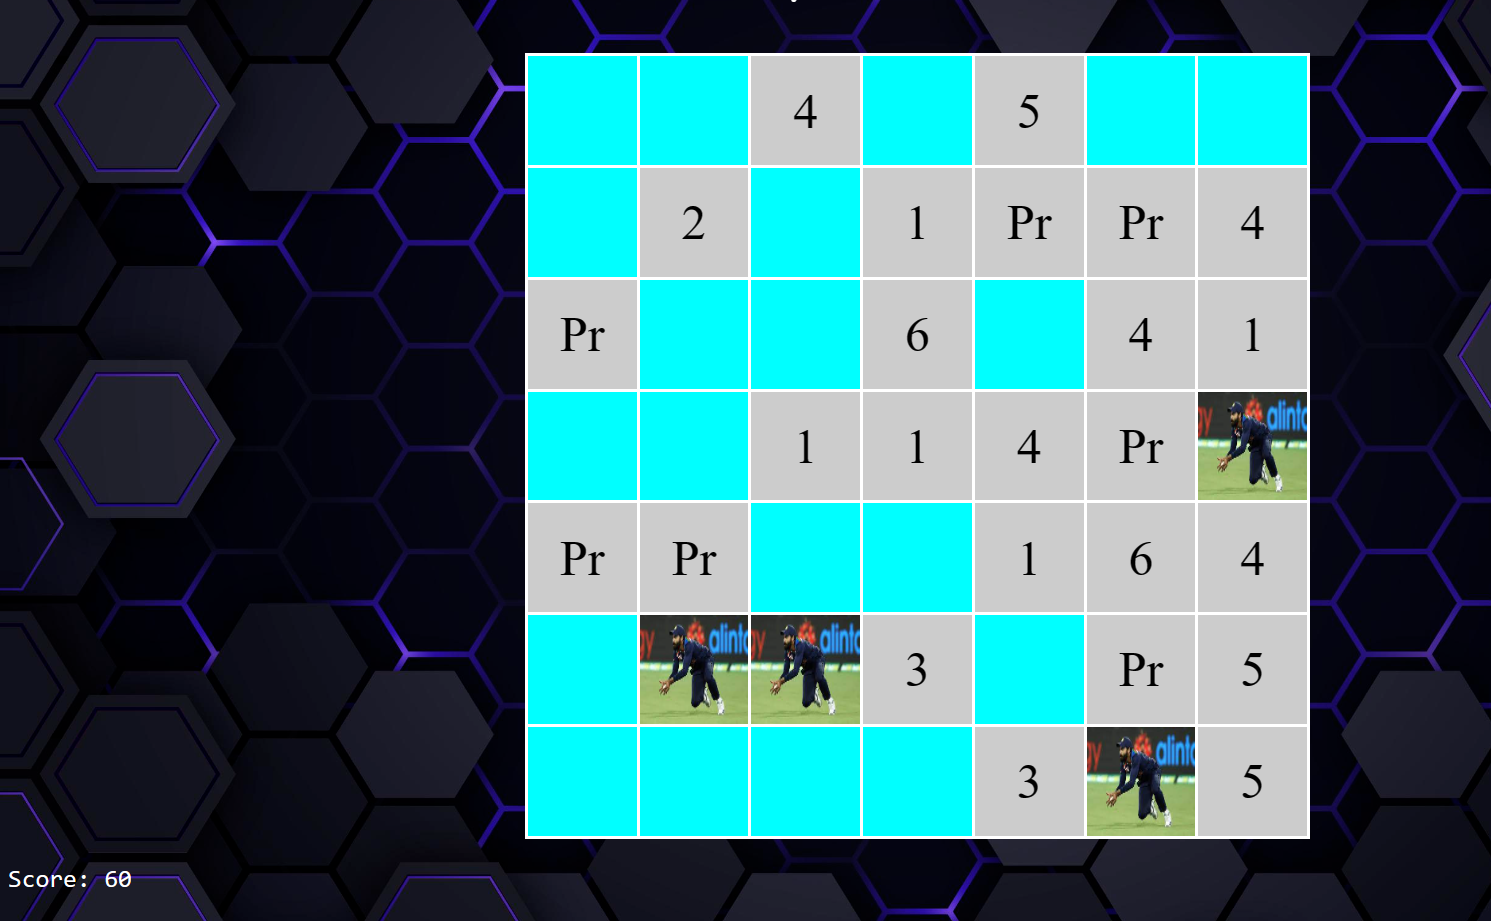
\includegraphics[width=0.8\textwidth]{image2.png}
    
    \item \textbf{Multiplier:}
    
    Apart from adding Protection, I have also added score multiplier property. If a player lands on such cell, his score gets twice. For this too I give the name of the attribute in the special characteristic of the cell. The number of such cells is limited in the game and is equal to the grid size.
    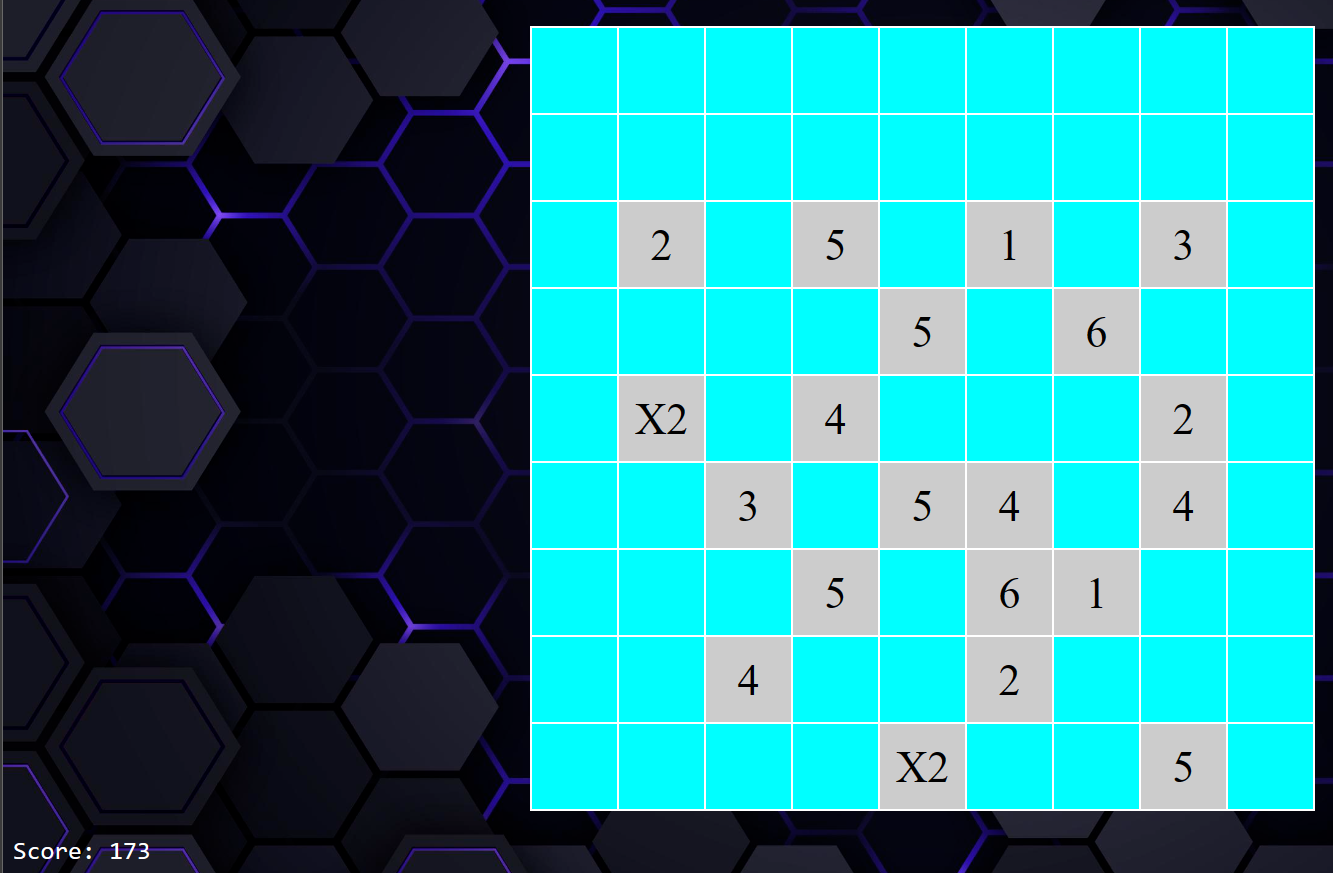
\includegraphics[width=0.8\textwidth]{image3.png}
    
\end{enumerate}

A player can start with either single player or multiplayer and can have none, one or both of the special attrubutes in the game.

Apart from these, when a player is playing, two new buttons appear in the bottom right of the page. The first button is for returning to the index page and starting a new game with different features. The second button is to start a new game with the same features.

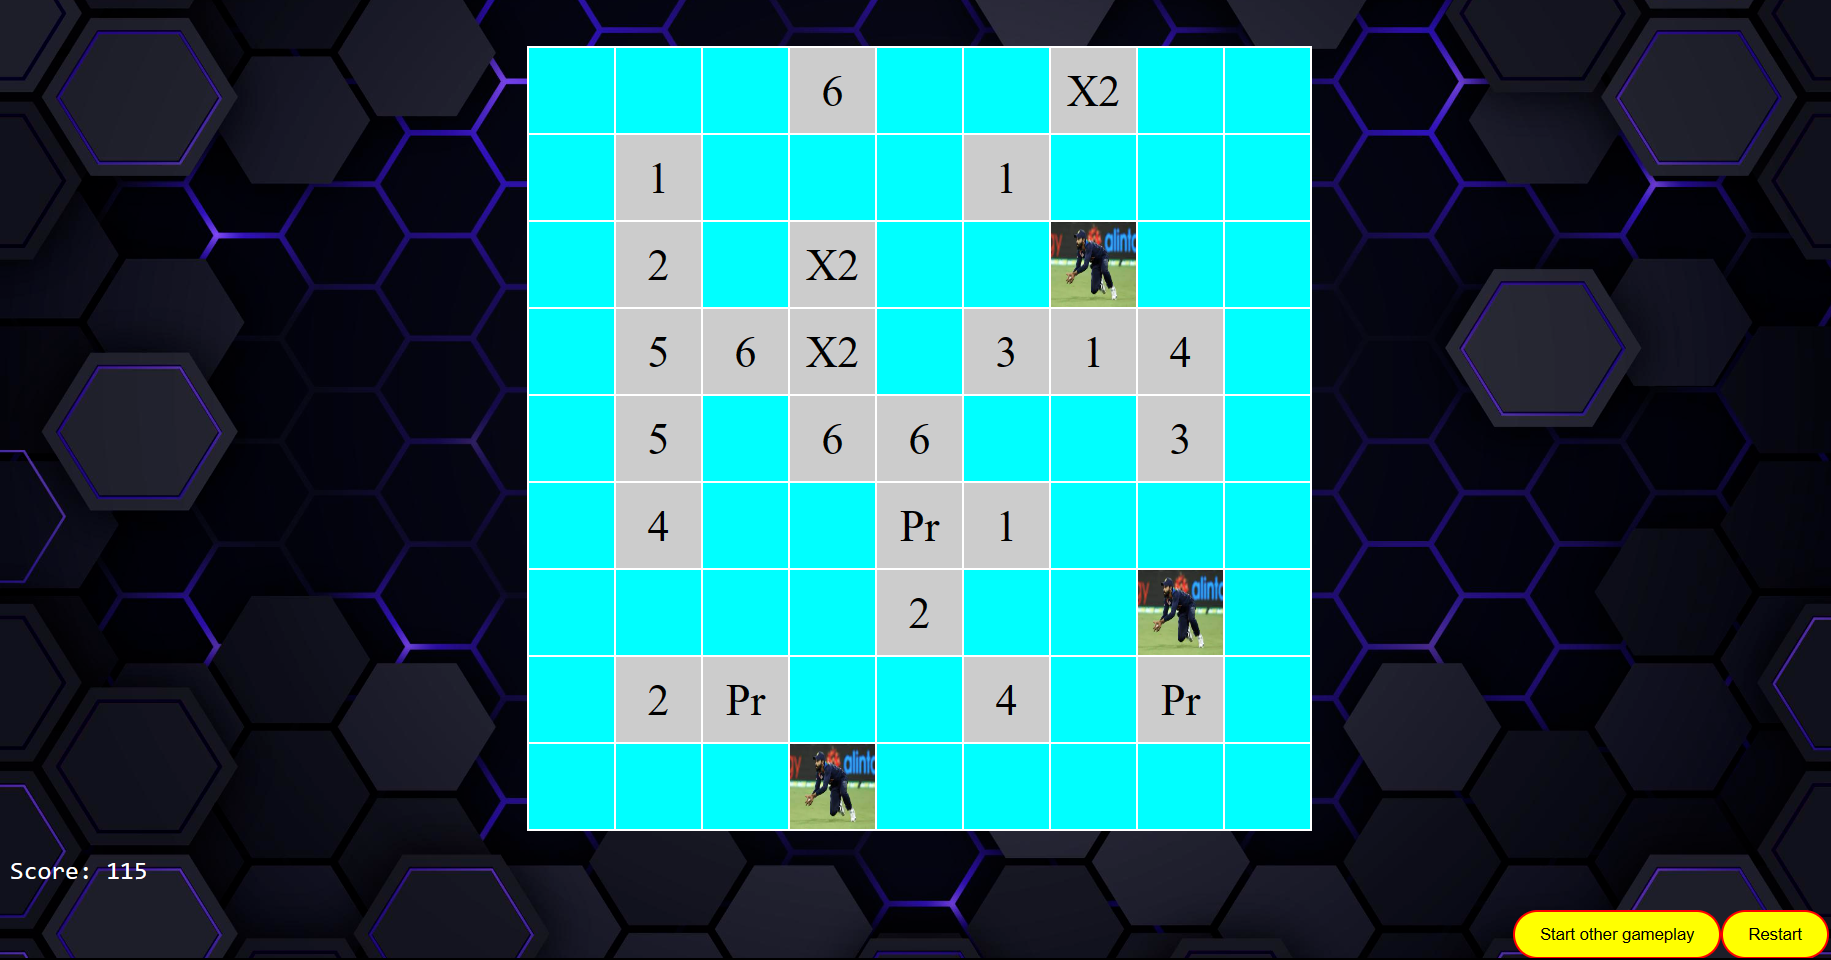
\includegraphics[width = 0.9\textwidth]{image4.png}

\newpage

\nocite{*}
\bibliographystyle{plain}
\bibliography{report}

\end{document}



% \begin{enumerate}
%     \item \textcolor{red}{\href{https://www.w3schools.com/js/}{W3Schools Tutorials}}
%     \item \textcolor{red}{\href{https://www.javatpoint.com/javascript-tutorial}{javaTpoint Tutorials}}
%     \item \textcolor{red}{\href{https://www.overleaf.com/learn/latex/Learn_LaTeX_in_30_minutes}{Overleaf Latex}}
%     \item Stack exchange
%     \item chatGPT
% \end{enumerate}